Die stochastische Kodierung nutzt ein zufällig generiertes Muster als Szene.
Geeignet für dieses Verfahren sind sogenannte \glqq Specklemuster\grqq ~\cite{specklePattern}.
Es handelt sich dabei um bandbegrenzte Muster mit zufällig verteilten Grauwerten.
Aufgrund der Unschärfe und dem Rauschen, welche in der Aufnahme durch eine Kamera einfließen, ist die Bandbegrenztheit notwendig um eine Dekodierung zu ermöglichen.
Abbildung \ref{img:speckleMuster} zeigt ein solches Muster.
%
\begin{figure}[H]
	\centering
	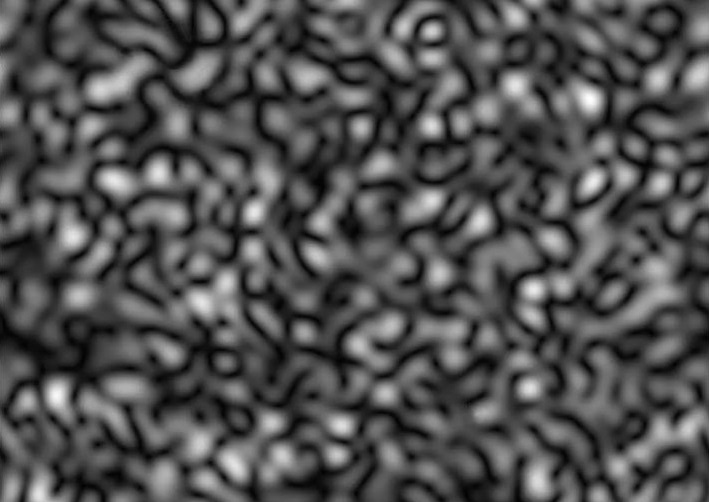
\includegraphics[frame,width=0.5\textwidth]{02_grundlagenZurDeflektometrie/rekonstruktion/stochastischeKodierung/figures/speckleMuster}
	\caption[Specklemuster]{Specklemuster.}
	\label{img:speckleMuster}
\end{figure}
%
\noindent
Das Grundprinzip der Dekodierung für dieses Kodierverfahren ist das Verfolgen der Punkte beim Verschieben des Specklemusters.
Es wird zunächst die Spiegelung des Specklemusters aufgenommen und ein Referenzpunkt definiert.
Nach der Verschiebung des Specklemusters (z. B. in x-Richtung) wird dieser Referenzpunkt in dem zweiten Bild über seine Umgebung gesucht.
Dabei verwendet man einen Algorithmus zur Berechnung der zweidimensionalen Bildkorrelation, die die höchste Übereinstimmung mit der Umgebung sucht.
Wenn der verschobene Referenzpunkt gefunden wurde, wird an derselben Stelle der Punkt im ersten Bild markiert.
Der markierte Punkt ist dann der neue Referenzpunkt, der im zweiten Bild gesucht wird.
Dieser Vorgang wiederholt sich, solange die Referenzpunkte im Bild liegen.
Abbildung \ref{img:prinzipStoKodierung} zeigt schematisch das Verfahren zur Dekodierung.
%
\begin{figure}[H]
	\centering
	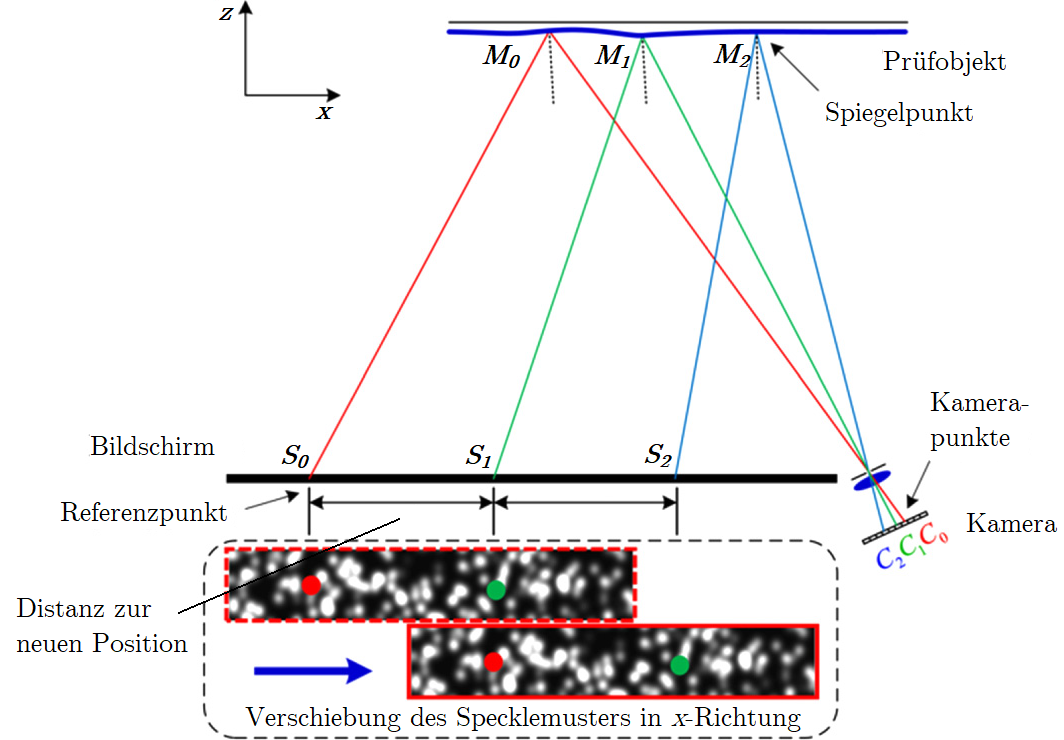
\includegraphics[width=0.9\textwidth]{02_grundlagenZurDeflektometrie/rekonstruktion/stochastischeKodierung/figures/Prinzip}
	\caption[Prinzip der Zuordnung einer stochastischen Kodierung]{Prinzip der Zuordnung einer stochastischen Kodierung. \textit{in Anlehnung an} \cite{specklePattern}}
	\label{img:prinzipStoKodierung}
\end{figure}
%
\noindent
Führt man dasselbe auch für die andere Richtung (z. B. in y-Richtung) durch, erhält man ein Raster auf dem Objekt, an dem die Objektpunkte zugeordnet wurden (siehe Abbildung \ref{img:ergebnisStoKodierung}).
%
\begin{figure}[H]
	\centering
	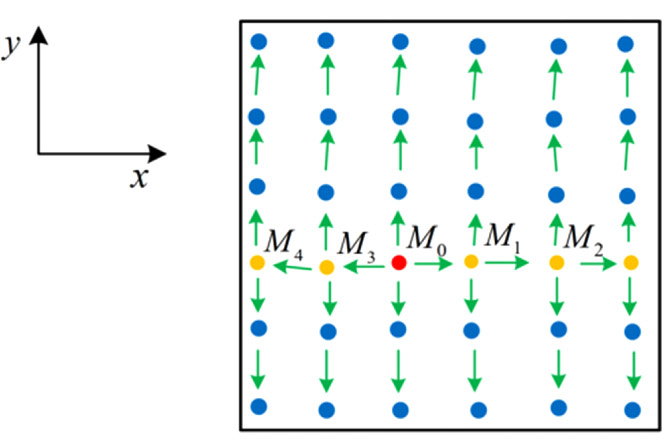
\includegraphics[width=0.4\textwidth]{02_grundlagenZurDeflektometrie/rekonstruktion/stochastischeKodierung/figures/Ergebnis}
	\caption[Ergebnis der Zuordnung einer stochastischen Kodierung]{Ergebnis der Zuordnung einer stochastischen Kodierung. Die grünen Pfeile zeigen an, von welchem Referenzpunkt man auf die nächste Zuordnung kam. \textit{in Anlehnung an} \cite{specklePattern}}
	\label{img:ergebnisStoKodierung}
\end{figure}
%
\noindent
Im Vergleich zu den vorgestellten Kodierverfahren in den vorherigen Abschnitten \ref{sub:phasenKodierung} und \ref{sub:frequenzKodierung}, liefert die Dekodierung in diesem Fall nur eine begrenzte Auflösung und keine vollflächige Zuordnung.
Außerdem ist dieses Verfahren nicht anwendbar für Objekte, die eine große Verzerrung der Musters erzeugen, da die zweidimensionalen Bildkorrelation ansonsten die Referenzpunkte nicht finden kann.
Dennoch sind die Vorteile dieses Verfahren der geringe Rechenaufwand und die Möglichkeit durch drei Bilder eine erfolgreiche Dekodierung durchzuführen \cite{specklePattern}.